% !TeX program = lualatex
\documentclass{article}
\usepackage[14pt]{extsizes}

% Begin embedded Chapter 1 preamble (edit packages and macros here).
\parindent 0em
\parskip0em
% Allow long mathematical terms to wrap without protruding into the margins.
\setlength{\emergencystretch}{2em}
\topmargin -2.0 truecm
\textheight 24 truecm
\textwidth 17.5 truecm
\oddsidemargin -1 truecm
\evensidemargin -1 truecm

% Times-style fonts for both pdfLaTeX and LuaLaTeX/XeLaTeX.
\usepackage{iftex}
\usepackage{amsmath}
\usepackage{enumerate}
\ifPDFTeX
  \usepackage[T1]{fontenc}
  \usepackage{tgtermes}
  \usepackage{newtxmath}
\else
  \usepackage{fontspec}
  \setmainfont{TeX Gyre Termes}
  \usepackage{unicode-math}
  \setmathfont{TeX Gyre Termes Math}
\fi
\usepackage{fancyhdr}
\usepackage{color}
\usepackage{graphicx}
\usepackage{pgf,tikz,pgfplots}
\pgfplotsset{compat=1.18}
\usetikzlibrary{arrows, shapes.geometric, matrix, turtle, plotmarks}
\usepackage{url}
\usepackage{xcolor}
\usepackage{dashrule}



%%%


\definecolor{answercolor}{RGB}{148,0,211}  % Purple color for answers
% Answer functionality
\newif\ifshowanswers
\showanswersfalse  % Default to hiding answers
% Command to show/hide answers
\newcommand{\printanswers}{\showanswerstrue}
\newcommand{\hideanswers}{\showanswersfalse}
% Answer Box Commands
% Usage:
%   \answer{math content}         - Creates box with default height (4cm)
%   \answer[6cm]{math content}    - Creates box with specified height
% The box height remains constant whether answers are shown or hidden
% (\printanswers or \hideanswers), ensuring consistent page layout.
\newcommand{\answer}[2][4cm]{%
	\noindent\framebox[\textwidth]{%
		\begin{minipage}[t][#1][t]{\dimexpr\textwidth-2\fboxsep-2\fboxrule\relax}
			\ifshowanswers
			{\color{answercolor}#2\par}
			\fi
		\end{minipage}%
	}
}
\newcommand\shortanswer[1]{%
	\ifshowanswers%
	\underline{\color{answercolor}{\hspace{0.5em} #1\hspace{0.5em}}}%
	\else%
	\underline{\phantom{\hspace{0.5em} #1\hspace{0.5em}}}%
	\fi%
}



\definecolor{fillincolor}{RGB}{148,0,211}  % Purple color for fillin-ins
% Fiil-in functionality
\newif\ifshowfillins
\showfillinsfalse  % Default to hiding answers
% Command to show/hide answers
\newcommand{\printfillins}{\showfillinstrue}
\newcommand{\hidefillins}{\showfillinsfalse}
\newcommand\fillin[1]{%
	\ifshowfillins%
	\underline{\color{fillincolor}{\hspace{0.5em} #1\hspace{0.5em}}}%
	\else%
	\underline{\phantom{\hspace{0.5em} #1\hspace{0.5em}}}%
	\fi%
}


%%%

\pagestyle{fancy}

\renewcommand{\headrulewidth}{0pt}
%\lhead{\tiny Math 345: Spring 2025, copyright: Lindsey, Zimmer, Roch}
\lhead{\tiny Math 345: Spring 2025, copyright: Phillipson, Roch}



\newcommand\displayspace[1]{\begin{multline*}
    \shoveright {#1}
    \end{multline*}}

\newcommand{\ruleone}{\rule{1in}{0.0005in}}
\newcommand{\ruleonepfive}{\rule{1.5in}{0.0005in}}
\newcommand{\ruletwo}{\rule{2in}{0.0005in}}

\newcommand{\hspaceone}{\hspace{1in}}

\newcommand{\bbR}{\mathbb{R}}

\newcommand{\calF}{{\mathcal{F}}}
\newcommand{\inv}{{^{-1}}}
\newcommand{\Ainv}{{A^{-1}}}
\newcommand{\by}{{\times}}

\DeclareMathOperator{\adj}{adj}
\DeclareMathOperator{\spn}{span}
\DeclareMathOperator{\rank}{rank}
\DeclareMathOperator{\nullity}{nullity}
\DeclareMathOperator{\Tr}{tr}
\DeclareMathOperator{\range}{range}
\DeclareMathOperator{\minor}{minor}
\DeclareMathOperator{\cof}{cof}
\DeclareMathOperator{\diag}{diag}
\DeclareMathOperator{\im}{im}
\DeclareMathOperator{\col}{col}
\DeclareMathOperator{\row}{row}
\DeclareMathOperator{\nool}{null}



\newcommand\ola[1]{\textcolor{magenta}{O: #1}}
\newcommand\peti[1]{\textcolor{teal}{P: #1}}
\newcommand\rub[1]{\textcolor{teal}{#1}}
\newcommand\points[1]{\textcolor{blue}{\textrm{+#1}}}

%%%%%%%%%%%%%%%%%%%
%%%headings etc.
%%%%%%%%%%%%%%%%%%%



\newcommand\notice{\textit{Notice:} }
\newcommand\question{\textbf{Question:} }
\newcommand\proof{\textbf{Why is it true?} }
\newcommand\setup{\textit{Set-up:} }
\newcommand\idea{\textit{Idea:} }
\newcommand\warning{\textbf{Warning:} }
\newcommand\topic[1]{\subsubsection*{#1}} 


% Create a common counter for all theorem-like environments
\newcounter{commoncount}

% Redefine the commands to use the counter
\newcommand\activity{\refstepcounter{commoncount}\textbf{Activity \thecommoncount:} }
\newcommand\theorem{\refstepcounter{commoncount}\textbf{Theorem \thecommoncount:} }
\newcommand\corollary{\refstepcounter{commoncount}\textbf{Corollary \thecommoncount:} }
\newcommand\lemma{\refstepcounter{commoncount}\textbf{Lemma \thecommoncount:} }
\newcommand\fact{\refstepcounter{commoncount}\textbf{Fact \thecommoncount:} }
\newcommand\note{\refstepcounter{commoncount}\textbf{Note \thecommoncount:} }
\newcommand\definition{\refstepcounter{commoncount}\textbf{Definition \thecommoncount:} }
\newcommand\remark{\refstepcounter{commoncount}\textit{Remark \thecommoncount:} }

% Section headings and PDF bookmarks.
\newcommand\sectiontitle[2]{\subsection*{Section #1: #2}%
  \addcontentsline{toc}{subsection}{Section #1: #2}}
\newcommand\chaptertitle[2]{\section*{Chapter #1: #2}%
  \addcontentsline{toc}{section}{Chapter #1: #2}}

% Boxed lecture material with breakable text and horizontal rules.
\newenvironment{framed}{\par\medskip\hrule\smallskip}
  {\par\smallskip\hrule\medskip}

%matrix entries 
\newcommand{\aaa}[2]{{a_{#1#2}}}
\newcommand{\aij}{{a_{ij}}}
\newcommand{\bbb}[2]{{b_{#1#2}}}
\newcommand{\bij}{{b_{ij}}}
\newcommand{\ccc}[2]{{c_{#1#2}}}
\newcommand{\cij}{{c_{ij}}}

%matrix minors and cofactors 
\newcommand{\Aij}{{A_{ij}}}
\newcommand{\Mij}{{M_{ij}}}


%dimension shortcuts 
\newcommand{\mbyn}{{m \times n}}
\newcommand{\nbyn}{{n \times n}}

%vectors 
\newcommand{\veca}{{\vec{a}}}
\newcommand{\bmata}{{\left[ \begin{array}{r} a_1 \\ a_2 \\ \ldots \\ a_n \end{array} \right] }}
\newcommand{\bmatb}{{\left[ \begin{array}{r} b_1 \\ b_2 \\ \ldots \\ b_n \end{array} \right] }}
\newcommand{\bmatx}{{\left[ \begin{array}{r} x_1 \\ x_2 \\ \ldots \\ x_n \end{bmatrix}{r} \right]}}

\newcommand{\colvec}[1]{{\left[ \begin{array}{r} #1 \end{array} \right]}}
\newcommand{\ccolvec}[1]{{\left[ \begin{array}{c} #1 \end{array} \right]}}
\newcommand{\twovec}[2]{{\left[ \begin{array}{r} #1 \\ #2 \end{array} \right]}}
\newcommand{\threevec}[3]{{\left[ \begin{array}{r} #1 \\ #2 \\ #3 \end{array} \right]}}
\newcommand{\fourvec}[4]{{\left[ \begin{array}{r} #1 \\ #2 \\ #3 \\ #4 \end{array} \right]}}

\newcommand{\colvecb}{{\left[ \begin{array}{c} b_1 \\ b_2 \\ \vdots \\ b_n \end{array} \right]}}
\newcommand{\colvecbm}{{\left[ \begin{array}{c} b_1 \\ b_2 \\ \vdots \\ b_m \end{array} \right]}}
\newcommand{\colvecc}{{\left[ \begin{array}{c} c_1 \\ c_2 \\ \vdots \\ c_n \end{array} \right]}}
\newcommand{\colvecx}{{\left[ \begin{array}{c} x_1 \\ x_2 \\ \vdots \\ x_n \end{array} \right]}}

\newcommand{\threerowvec}[3]{{\left[ \begin{array}{rrr} #1 & #2 & #3 \end{array} \right]}}
\newcommand{\fourrowvec}[4]{{\left[ \begin{array}{rrr} #1 & #2 & #3 & #4 \end{array} \right]}}

%matrix commands 
\newcommand{\twobytwo}[4]{{\left[ \begin{array}{rr} #1 & #2 \\ #3 & #4 \end{array} \right]}}
\newcommand{\cIthree}[1]{{\left[ \begin{array}{rrr} #1 & 0 & 0 \\ 0 & #1 & 0 \\ 0 & 0 & #1 \end{array} \right]}}
\newcommand{\barray}[2]{{\left[ \begin{array}{#1} #2 \end{array} \right]}}
\newcommand{\Amn}{{\left[ \begin{array}{cccc} 
a_{11} & a_{12} & \cdots & a_{1n} \\ 
a_{21} & a_{22} & \cdots & a_{2n} \\ 
\vdots & \vdots & \ddots & \vdots \\ 
a_{m1} & a_{m2} & \cdots & a_{mn}
\end{array} \right]}}
\newcommand{\Ann}{{\left[ \begin{array}{cccc} 
a_{11} & a_{12} & \cdots & a_{1n} \\ 
a_{21} & a_{22} & \cdots & a_{2n} \\ 
\vdots & \vdots & \ddots & \vdots \\ 
a_{n1} & a_{n2} & \cdots & a_{nn}
\end{array} \right]}}
\newcommand{\Amnb}{{\left[ \begin{array}{cccc|c} 
a_{11} & a_{12} & \cdots & a_{1n} & b_1 \\ 
a_{21} & a_{22} & \cdots & a_{2n} & b_2 \\ 
\vdots & \vdots & & \vdots & \vdots \\ 
a_{m1} & a_{m2} & \cdots & a_{mn} & b_m
\end{array} \right]}}

%math boldface

\newcommand{\bfa}{{\mathbf{a}}}
\newcommand{\bfb}{{\mathbf{b}}}
\newcommand{\bfc}{{\mathbf{c}}}
\newcommand{\bfd}{{\mathbf{d}}}
\newcommand{\bfe}{{\mathbf{e}}}
\newcommand{\bff}{{\mathbf{f}}}
\newcommand{\bfi}{{\mathbf{i}}}
\newcommand{\bfj}{{\mathbf{j}}}
\newcommand{\bfk}{{\mathbf{k}}}
\newcommand{\bfu}{{\mathbf{u}}}
\newcommand{\bfv}{{\mathbf{v}}}
\newcommand{\bfw}{{\mathbf{w}}}
\newcommand{\bfx}{{\mathbf{x}}}
\newcommand{\bfy}{{\mathbf{y}}}
\newcommand{\bfz}{{\mathbf{z}}}
\newcommand{\bfzero}{{\mathbf{0}}}
\newcommand{\bfone}{{\mathbf{1}}}


%%%%%%%%%%%%%%%%%%%%
%%%DASH LINE COMMAND
%%%%%%%%%%%%%%%%%%%%

\makeatletter
\newcommand*\dashline{\mathrel{\vert}}
\makeatother

%%%%%%%%%%%%%%%%%%%%
%%%INTEGRAL
%%%%%%%%%%%%%%%%%%%%

\newcommand{\ddd}{\mathrm{d}}

%%%%%%%%%%%%%%%%%%%
%%%%  TIKZ %%%%%%%%
%%%%%%%%%%%%%%%%%%%

\newcommand{\coordsys}[4]{
\foreach \x in {#1,...,#3}
\draw[line width=.6pt,color=black!15,dashed] (\x,#2-.2) -- (\x,#4+.2);
\foreach \y in {#2,...,#4}
\draw[line width=.6pt,color=black!15,dashed] (#1-.2,\y) -- (#3+.2,\y);
\draw[->] (#1-.2,0) -- (#3+.2,0) node[right] {$x$};
\draw[->] (0,#2-.2) -- (0,#4+.2) node[above] {$y$};
\foreach \x in {#1,...,-1}
\draw[shift={(\x,0)},color=black] (0pt,2pt) -- (0pt,-2pt) node[below] {\footnotesize $\x$};
\foreach \x in {1,...,#3}
\draw[shift={(\x,0)},color=black] (0pt,2pt) -- (0pt,-2pt) node[below] {\footnotesize $\x$};
\foreach \y in {#2,...,-1}
\draw[shift={(0,\y)},color=black] (2pt,0pt) -- (-2pt,0pt) node[left] {\footnotesize $\y$};
\foreach \y in {1,...,#4}
\draw[shift={(0,\y)},color=black] (2pt,0pt) -- (-2pt,0pt) node[left] {\footnotesize $\y$};
}


%%%

% PDF links and document information
\usepackage{hyperref}
\hypersetup{
	pdftitle={Math 345 - Chapter 1: Systems of Linear Equations},
	pdfauthor={Sebastien Roch},
	pdfsubject={Linear algebra and optimization},
	pdfkeywords={linear algebra, lecture notes, mathematics},
	pdfstartview=Fit,
	pdfinfo={
		Title={Math 345 - Chapter 1: Systems of Linear Equations}
	}
}
% End embedded Chapter 1 preamble.

% Commands to show/hide answers/fillins
% Uncomment if needed
% Default is hiding
\printanswers
\printfillins

\begin{document}


\chaptertitle{1}{Systems of Linear Equations}
{\small These notes use material from your textbook \textit{Linear Algebra with Applications} by W. Keith Nicholson [LAWA]. Sections are numbered in their order of presentation within each chapter.}

\bigskip

Learning goals:
	\begin{itemize}
		\item Be able to set up an augmented matrix for a linear system of equations and be able to
		interpret an augmented matrix as a linear system of equations
		\item Be able to perform elementary row operations to a matrix
		\item Know how to find a REF or the RREF form for a matrix
		\item Be able to solve linear system using the method of Gaussian Elimination
		\item Be able to find the rank of a matrix and know what it tells you about the number of
		solutions for the corresponding linear system
		\item Know how to build the basic solutions for a homogeneous system
		\item Know how to determine the number of basic solutions of a homogeneous system using
		the rank		
	\end{itemize}

%\bigskip	
\newpage


\sectiontitle{1.1}{Solutions and Elementary Operations} 

\remark Codex is fun!

\activity In a Wisconsin forest, there are robins and badgers. Together they have 18 heads and 56 legs. How many robins and badgers are in the forest? 

\answer[12cm]{
$x$ = number of robins, $y$ = number of badgers
\begin{align*}
x + y &= 18 \quad \text{(heads)} \\
2x + 4y &= 56 \quad \text{(legs)}
\end{align*}
From first equation: $y = 18-x$\\
Substitute into second:
\begin{align*}
2x + 4(18-x) &= 56 \\
2x + 72 - 4x &= 56 \\
-2x &= -16 \\
x &= 8 \quad \text{robins} \\
y &= 10 \quad \text{badgers}
\end{align*}
}


\bigskip

An equation of the form 
$$ a_1 x_1 + a_2 x_2 + \cdots + a_n x_n = b $$
is called a \fillin{linear equation}. The real quantities $a_1, \ldots, a_n, b$ are \fillin{constants}, while the variables $x_1, \ldots, x_n$ represent \fillin{unknowns}.

%\bigskip
\newpage

\activity Identify the constants and unknowns in each linear equation in the first activity. 

\answer{
	\begin{align*}
		x + y &= 18: & \text{constants} \; 1,1,18; & \text{ unknowns} \; x,y \\
		2x + 4y &= 56: & \text{constants} \; 2,4,56; & \text{ unknowns} \; x,y
	\end{align*}
}

\bigskip

\activity What are some equations that are not linear equations? 

\answer[6cm]{
\begin{itemize}
	\item $x^2 + y = 1$ (contains squared term)
	\item $xy = 2$ (contains product of variables) 
	\item $\sin(x) + y = 0$ (contains trigonometric function)
	\item $\sqrt{x} + y = 1$ (contains square root)
\end{itemize}
}

\bigskip

More generally, a \fillin{system of linear equations} or \fillin{linear system} is a set of $m$ linear equations each in $n$ unknowns. A linear system has the form 
\[
\begin{array}{lllllll}
a_{11}x_1 + & a_{12}x_2 + & \cdots + & a_{1n}x_n & = & b_1 & \\
a_{21}x_1 + & a_{22}x_2 + & \cdots + & a_{2n}x_n & = & b_2 & \\ 
\vdots & \vdots & & \vdots & & \vdots & (*) \\ 
a_{m1}x_1 + & a_{m2}x_2 + & \cdots + & a_{mn}x_n & = & b_m. & 
\end{array}
\]
A \fillin{solution} to the linear system $(*)$ is a sequence of $n$ numbers $s_1, \ldots, s_n$ so that \textit{each} equation in $(*)$ is satisfied when $x_1 = s_1$, $x_2 = s_2$, $\ldots$, $x_n = s_n$ are substituted. 

\bigskip

Let $(*)$ be a linear system as above. 
\begin{itemize}
    \item If $(*)$ has \textit{no} solution, it is called \fillin{inconsistent}. 
    \item If $(*)$ has a solution, it is called \fillin{consistent}. (Note that it may have infinitely many solutions!)
    \item If $(*)$ has $b_1 = b_2 = \cdots = b_n = 0$, it is called a \fillin{homogeneous system}. 
        \begin{itemize}
            \item Note that $x_1 = x_2 = \cdots = x_n = 0$  is always a solution to a homogeneous system. It is called the \fillin{trivial} solution.
            \item A solution to a homogeneous system where \textit{not} each $x_i$ is $0$ is called a \fillin{nontrivial} solution. 
        \end{itemize}
\end{itemize}

Consider another system of $r$ linear equations in $n$ unknowns: 
\[
\begin{array}{lllllll}
c_{11}x_1 + & c_{12}x_2 + & \cdots + & c_{1n}x_n & = & d_1 & \\
c_{21}x_1 + & c_{22}x_2 + & \cdots + & c_{2n}x_n & = & d_2 & \\ 
\vdots & \vdots & & \vdots & & \vdots & (**) \\ 
c_{r1}x_1 + & c_{r2}x_2 + & \cdots + & c_{rn}x_n & = & d_r. & 
\end{array}
\]
The systems $(*)$ and $(**)$ are \fillin{equivalent} if they have exactly the same solutions. 

\bigskip

\note In $3d$ space, i.e., in three variables or unknowns, lines and planes are examples of systems of linear equations with inifinitely many solutions. When two distinct planes are parallel, i.e., when their normal vector is parallel, the intersection is empty---put differently, no solutions exist to the system of equations made of the equations in general form. 

%\bigskip
\newpage

\activity In another Wisconsin forest, there are also robins and badgers. Together they have 18 heads, 36 eyes, and 56 legs. How many robins and badgers are in the forest? Can we use any new terminology to describe this system? 


\answer[16cm]{
$x$ = number of robins, $y$ = number of badgers
\begin{align*}
	x + y &= 18 \quad \text{(heads)} \\
	2x + 2y &= 36 \quad \text{(eyes)} \\
	2x + 4y &= 56 \quad \text{(legs)}
\end{align*}
Note that second equation gives $x + y = 18$ (after dividing each side by $2$), same as first equation.

From first equation: $y = 18-x$

Substitute into third:
\begin{align*}
	2x + 4(18-x) &= 56 \\
	2x + 72 - 4x &= 56 \\
	-2x &= -16 \\
	x &= 8 \quad \text{robins} \\
	y &= 18 - 8 = 10 \quad \text{badgers}
\end{align*}
This is a system of three linear equations in two unknowns. It is consistent.	
}

%\bigskip
\newpage


\activity In a third Wisconsin forest, there are deer and badgers. Together they have 18 heads and 70 legs. How many deer and badgers are in the forest? Can we use any new terminology to describe this system? 


\answer[10cm]{
	$x$ = number of deer, $y$ = number of badgers
	\begin{align*}
		x + y &= 18 \quad \text{(heads)} \\
		4x + 4y &= 70 \quad \text{(legs)}
	\end{align*}
	From second equation:
	\begin{align*}
		4(x + y) &= 70 \\
		x + y &= \frac{70}{4} = 17.5
	\end{align*}
	This system is inconsistent since first equation gives $x + y = 18$ but second gives $x + y = 17.5$ (Try substituting the first equation into the second one.)
}

\bigskip

\theorem The following operations, called \fillin{elementary operations}, can be performed on systems of linear equations to produce \fillin{equivalent} systems.
\begin{enumerate}
    \item \fillin{Interchange} the $i$th and $j$th equations. 
    \item \fillin{Multiply} an equation by a nonzero constant. 
    \item \fillin{Replace} the $i$th equation by $c$ times the $j$th equation \textit{plus} the $i$th equation. 
\end{enumerate}

We can track these operations more easily using an array/matrix to record the coefficients. The \fillin{coefficient matrix} of the linear system is the $m\times n$ matrix $A$:

 \begin{minipage}{.48\textwidth}
 \[
\begin{array}{llllll}
a_{11}x_1 + & a_{12}x_2 + & \cdots + & a_{1n}x_n & = & b_1 \\
a_{21}x_1 + & a_{22}x_2 + & \cdots + & a_{2n}x_n & = & b_2 \\ 
\vdots & \vdots & & \vdots & & \vdots \\ 
a_{m1}x_1 + & a_{m2}x_2 + & \cdots + & a_{mn}x_n & = & b_m
\end{array}
\]
\end{minipage}
 \begin{minipage}{.03\textwidth}
\quad
\end{minipage}
 \begin{minipage}{.46\textwidth}
 \[
A = \begin{bmatrix}
\aaa11 & \aaa12 & \cdots & \cdots & \cdots & \aaa1n \\ 
\aaa21 & \aaa22 & \cdots & \cdots & \cdots & \aaa2n \\ 
\vdots & \vdots & \cdots & \cdots & \cdots & \vdots  \\ 
\vdots & \vdots & \cdots & \cdots & \cdots & \vdots \\ 
a_{m1} & a_{m2} & \cdots & \cdots & \cdots & a_{mn} \\ 
\end{bmatrix} 
\]
\end{minipage}

\vspace{0.15in}


We can also build a matrix that includes the constants on the right-hand side of the linear system. First, note that

$$\mathbf{b}=\begin{bmatrix} b_1 \\ b_2 \\ \vdots \\ b_m\end{bmatrix}$$

is a $m \times 1$ matrix (called the \fillin{constant matrix}) representing the constant terms of the linear equations (this is also called a \fillin{vector} or \fillin{column vector}). We can adjoin $\mathbf{b}$ to matrix $A$ to create the \fillin{augmented matrix} representing our linear system:


$$ [A \dashline \bfb]=
\Amnb
$$


\bigskip

\activity Consider the linear system 
\[ 
\begin{array}{rrrrrrr}
	&  & y & - & z & = & 4  \\
	2x & + & &  & 6z & = & 4 \\ 
	3x & + & 2y & + & 2z & = & -1
\end{array}
\]
The system is reduced to a simpler system using elementary operations.
Find the augmented matrix for the linear systems, then record the resulting matrices.

\answer{Initial augmented matrix:
	\[
	\left[\begin{array}{ccc|c}
		0 & 1 & -1 & 4 \\
		2 & 0 & 6 & 4 \\
		3 & 2 & 2 & -1
	\end{array}\right]
	\]
}

\shortanswer{Interchange rows 1 and 2:}
\[ 
\begin{array}{rrrrrrr}
	2x & + & &  & 6z & = & 4 \\ 
	&  & y & - & z & = & 4  \\
	3x & + & 2y & + & 2z & = & -1
\end{array}
\]

\answer{
	\[
	\left[\begin{array}{ccc|c}
		2 & 0 & 6 & 4 \\
		0 & 1 & -1 & 4 \\
		3 & 2 & 2 & -1
	\end{array}\right]
	\]
}

\shortanswer{Divide first row by 2:}
\[ 
\begin{array}{rrrrrrr}
	x & + & &  & 3z & = & 2\\ 
	&  & y & - & z & = & 4  \\
	3x & + & 2y & + & 2z & = & -1
\end{array}
\]

\answer{
	\[
	\left[\begin{array}{ccc|c}
		1 & 0 & 3 & 2 \\
		0 & 1 & -1 & 4 \\
		3 & 2 & 2 & -1
	\end{array}\right]
	\]
}

\shortanswer{Replace row 3 by row 3 - 3(row 1):}
\[ 
\begin{array}{rrrrrrr}
	x & + & &  & 3z & = & 2\\ 
	&  & y & - & z & = & 4  \\
	&  & 2y & - & 7z & = & -7
\end{array}
\]

\answer{
	\[
	\left[\begin{array}{ccc|c}
		1 & 0 & 3 & 2 \\
		0 & 1 & -1 & 4 \\
		0 & 2 & -7 & -7
	\end{array}\right]
	\]
}

\shortanswer{Replace row 3 by row 3 - 2(row 2):}
\[ 
\begin{array}{rrrrrrr}
	x & + & &  & 3z & = & 2\\ 
	&  & y & - & z & = & 4  \\
	&  & & - & 5z & = & -15
\end{array}
\]

\answer{
	\[
	\left[\begin{array}{ccc|c}
		1 & 0 & 3 & 2 \\
		0 & 1 & -1 & 4 \\
		0 & 0 & -5 & -15
	\end{array}\right]
	\]
}

\shortanswer{Multiply row 3 by -1/5:}
\[ 
\begin{array}{rrrrrrr}
	x & + & &  & 3z & = & 2\\ 
	&  & y & - & z & = & 4  \\
	&  & & & z & = & 3
\end{array}
\]

\answer{
	\[
	\left[\begin{array}{ccc|c}
		1 & 0 & 3 & 2 \\
		0 & 1 & -1 & 4 \\
		0 & 0 & 1 & 3
	\end{array}\right]
	\]
}

\shortanswer{Replace row 2 by row 2 + row 3:}
\[ 
\begin{array}{rrrrrrr}
	x & + & &  & 3z & = & 2\\ 
	&  & y &  &  & = & 7 \\
	&  & & & z & = & 3
\end{array}
\]

\answer{
	\[
	\left[\begin{array}{ccc|c}
		1 & 0 & 3 & 2 \\
		0 & 1 & 0 & 7 \\
		0 & 0 & 1 & 3
	\end{array}\right]
	\]
}

\shortanswer{Replace row 1 by row 1 - 3(row 3):}
\[ 
\begin{array}{rrrrrrr}
	x &  & &  & & = & -7\\ 
	&  & y &  &  & = & 7 \\
	&  & & & z & = & 3
\end{array}
\]

\answer{
	\[
	\left[\begin{array}{ccc|c}
		1 & 0 & 0 & -7 \\
		0 & 1 & 0 & 7 \\
		0 & 0 & 1 & 3
	\end{array}\right]
	\]
}


\bigskip

Notice that when we apply the elementary operations to the matrix, they change the rows of the matrix. 

\bigskip

\definition An \fillin{elementary row operation} on a matrix $A$ is any one of the following operations: 
\begin{enumerate}[(a)]
    \item Type I: \fillin{Interchange} any two rows.
    \item Type II: \fillin{Multiply} a row by a nonzero number. 
    \item Type III: \fillin{Add} a multiple of one row to another. 
\end{enumerate}


\bigskip

\noindent\textbf{Geometric Point of View---Explore on Own!}  Consider the following three systems, inspired by our forest activities. Graph the lines defined by these equations and check how this reflects the number of solutions in each case.

\begin{minipage}{0.3\textwidth}
\[\begin{array}{rrrrr}
x & + & y & = & 18 \\ 
2x & + & 4y & = & 56 \\
\end{array}\]
\end{minipage}
%
\begin{minipage}{0.3\textwidth}
\[\begin{array}{rrrrr}
x & + & y & = & 18 \\ 
4x & + & 4y & = & 72 \\
\end{array}\]
\end{minipage}
%
\begin{minipage}{0.3\textwidth}
\[\begin{array}{rrrrr}
x & + & y & = & 18 \\ 
4x & + & 4y & = & 56 \\
\end{array}\]
\end{minipage}

%\bigskip
\newpage

\sectiontitle{1.2}{Gaussian Elimination}

\activity The following are augmented matrices representing systems of linear equations in three unknowns ($x, y, z$). Rewrite the equations, then solve the systems.

(a) $ \left[ \begin {array}{cccc} 1&2&1&4\\ \noalign{\medskip}0&1&2&2
\\ \noalign{\medskip}0&0&1&-2\end {array} \right] $

\bigskip

\answer[10cm]{
Rewrite as:
\[
\begin{aligned}
	x + 2y + z &= 4 \\
	y + 2z &= 2 \\
	z &= -2
\end{aligned}
\]
Back substitution:
\[
\begin{aligned}
	z &= -2 \\
	y + 2(-2) &= 2 \implies y = 6 \\
	x + 2(6) + (-2) &= 4 \implies x = -6
\end{aligned}
\]
Solution: $x = -6$, $y = 6$, $z = -2$.
}

\bigskip

(b) $ \left[ \begin {array}{cccc} 1&0&0&-5\\ \noalign{\medskip}0&1&0&2
\\ \noalign{\medskip}0&0&1&4\end {array} \right]$

\bigskip

\answer[6cm]{
Rewrite as:
\[
\begin{aligned}
	x &= -5 \\
	y &= 2 \\
	z &= 4
\end{aligned}
\]
Solution: $x = -5$, $y = 2$, $z = 4$.
}

\bigskip

\definition An $\mbyn$ matrix $A$ is in \fillin{row echelon form} (REF) if it satisfies the following properties: 
\begin{enumerate}[(a)]
    \item All \fillin{zero rows}, if there are any, appear at the \fillin{bottom} of the matrix. 
    \item The \fillin{first nonzero entry} from the left of a nonzero row is a 1. This entry is called the \fillin{leading one} of its row. 
    \item For each nonzero row, the leading one appears to the \fillin{right and below} any leading ones in \fillin{preceding} rows. 
\end{enumerate}
We say $A$ is in \fillin{reduced row echelon form} (RREF) if $A$ is in REF and also satisfies 
\begin{enumerate}
    \item[(d)] If a column contains a leading one, then \fillin{all other entries} in that column are zero. 
\end{enumerate}

\bigskip



A matrix in REF appears as a staircase (or \fillin{echelon}) pattern of leading ones descending from the upper left corner of the matrix. Let's draw a schematic of a matrix in REF.

\begin{figure}[!h]
	\centering
	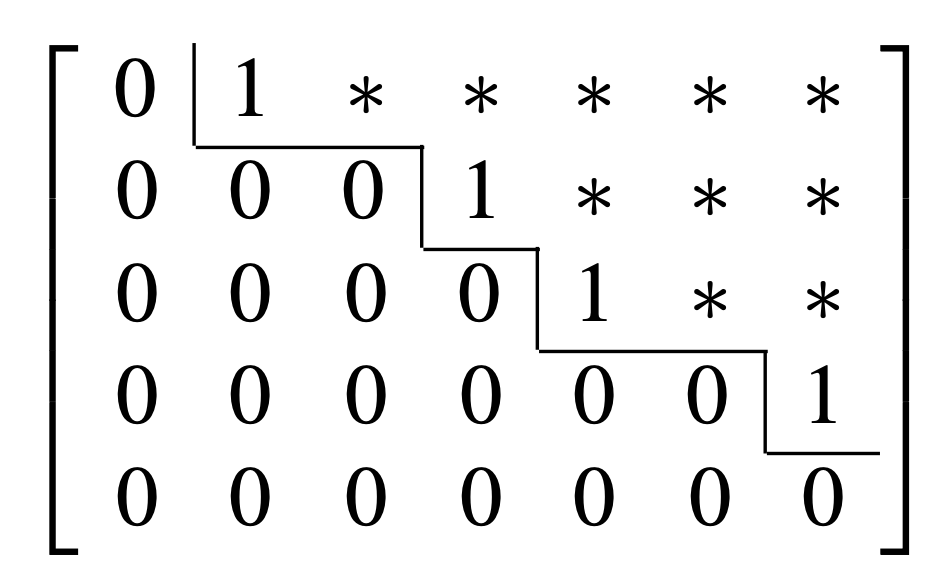
\includegraphics[width=3in]{staircase}
	\caption{From Linear Algebra with Applications, Vretta-Lyryx}
\end{figure}


\bigskip

\activity Which of the following matrices are in REF? Which are in RREF?

\bigskip 

$A = \barray{ccccc}{1 & 3 & 0 & 0 & 1 \\ 0 & 0 & 1 & 3 & 2 \\ 0 & 0 & 0 & 0 & 0}$ 

\smallskip

\shortanswer{Both REF and RREF (staircase, 0s in columns with leading 1s)}

\bigskip

$B = \barray{cccc}{1 & 4 & 0 & 2 \\ 0 & 0 & 0 & 0 \\ 0 & 0 & 1 & -2}$ 
\smallskip

\shortanswer{Not REF (zero row not at bottom)}

\bigskip

$C = \barray{rrrr}{1 & 3 & 5 & 7 \\ 0 & 1 & -1 & 5 \\ 0 & 0 & 1 & 10 \\ 0 & 0 & 0 & 0}$ 
\smallskip

\shortanswer{REF but not RREF (has nonzero entries above leading 1s)}

\bigskip


$D = \barray{rrrrr}{1 & 0 & 0 & 0 & -1 \\ 0 & 1 & 0 & 0 & 4 \\ 0 & 0 & 0 & 1 & 6}$ 
\smallskip

\shortanswer{Both REF and RREF (has zeros above and below leading 1s)}

\bigskip

$E = \barray{rrrr}{1 & 0 & 4 & 3 \\ 0 & 1 & 2 & 2 \\ 0 & 1 & -5 & 2 \\ 0 & 0 & 0 & 0}$ 
\smallskip

\shortanswer{Not REF (third row has leading 1 in same column as second row)}

\bigskip


\definition For a matrix in REF, the first 1 that appears in a row is called a \fillin{pivot}. The columns containing pivots are called \fillin{pivot columns}.

\bigskip

\definition An $m \times n$ matrix $A$ is \fillin{row equivalent} to an $m \times n$ matrix $B$ if $B$ can be produced by applying a finite sequence of elementary row operations to $A$. 

\bigskip 

\theorem Every $\mbyn$ matrix $A$ is \fillin{row equivalent} to a \fillin{unique} matrix in RREF. 

%\bigskip 
\newpage

\begin{framed}\textbf{Gaussian Algorithm: How to find a row-echelon matrix from a given matrix}

\textit{Heuristic}: Move from top to bottom and outside in until you get an upper triangular-ish matrix with ones as leading entries. 

\begin{itemize}
\item[1.] If the matrix consists entirely of zeros, stop—it is already in row-echelon form.
\item[2.] Otherwise, find the first column from the left containing a nonzero entry (call it $a$), and move the row containing that entry to the top position.
\item[3.] Now multiply the new top row by $1/a$ to create a leading 1.
\item[4.] By subtracting multiples of that row from rows below it, make each entry below the leading 1 zero.

\end{itemize}
This completes the first row, and all further row operations are carried out on the remaining rows.

\begin{itemize}
\item[5.] Repeat steps 1–4 on the matrix consisting of the remaining rows.
\end{itemize}

The process stops when either no rows remain at step 5 or the remaining rows consist entirely of
zeros.

\end{framed}

%\bigskip
\newpage

\activity Find a row echelon form of the given matrix $A$. 

$$
A = \barray{rrrr}{0 & 0 & 1 & 2 \\ 3 & 3 & 6 & -9 \\ 2 & 3 & 0 & -2}
$$

\answer[14cm]{
First nonzero column is column 1. Interchange rows 1 and 2:
$ \barray{rrrr}{3 & 3 & 6 & -9 \\ 0 & 0 & 1 & 2 \\ 2 & 3 & 0 & -2} $

Multiply first row by 1/3:
$ \barray{rrrr}{1 & 1 & 2 & -3 \\ 0 & 0 & 1 & 2 \\ 2 & 3 & 0 & -2} $

Subtract 2 times first row from row 3:
$ \barray{rrrr}{1 & 1 & 2 & -3 \\ 0 & 0 & 1 & 2 \\ 0 & 1 & -4 & 4} $

Interchange rows 2 and 3:
$ \barray{rrrr}{1 & 1 & 2 & -3 \\ 0 & 1 & -4 & 4 \\ 0 & 0 & 1 & 2} $

Matrix is now in REF with leading 1s in columns 1, 2, and 3.}

\bigskip 

%\textit{Note}: The elementary row operations applied to $A$ to put it in RREF might not be unique, but the RREF matrix obtained at the end is. 



\theorem Consider two linear systems each of $m$ equations in $n$ unknowns. If the augmented matrices $[A \dashline b]$ and $[C \dashline d]$ are \fillin{row equivalent}, then the linear systems are \fillin{equivalent}, i.e. the systems have the same solutions. 


\bigskip 


\activity Solve the linear system 
\[
\begin{array}{rrrrrrr}
    x & + & 2y & + & 3z & = & 9 \\
    2x & - & y & + & z & = & 8 \\
    3x & & & - & z & = & 3
\end{array}
\]
by transforming the associated matrix $[A \dashline \bfb]$ to row echelon form. 

\answer[23.5cm]{
Augmented matrix:
$$ \left[ \begin{array}{rrr|r} 
	1 & 2 & 3 & 9 \\
	2 & -1 & 1 & 8 \\
	3 & 0 & -1 & 3
\end{array} \right] $$

Subtract 2 times row 1 from row 2 and
%$$ \left[ \begin{array}{rrr|r}
%	1 & 2 & 3 & 9 \\
%	0 & -5 & -5 & -10 \\
%	3 & 0 & -1 & 3
%\end{array} \right] $$
%
subtract 3 times row 1 from row 3:
$$ \left[ \begin{array}{rrr|r}
	1 & 2 & 3 & 9 \\
	0 & -5 & -5 & -10 \\
	0 & -6 & -10 & -24
\end{array} \right] $$

Multiply row 2 by -1/5:
$$ \left[ \begin{array}{rrr|r}
	1 & 2 & 3 & 9 \\
	0 & 1 & 1 & 2 \\
	0 & -6 & -10 & -24
\end{array} \right] $$

Add 6 times row 2 to row 3:
$$ \left[ \begin{array}{rrr|r}
	1 & 2 & 3 & 9 \\
	0 & 1 & 1 & 2 \\
	0 & 0 & -4 & -12
\end{array} \right] $$

Multiply row 3 by -1/4:
$$ \left[ \begin{array}{rrr|r}
	1 & 2 & 3 & 9 \\
	0 & 1 & 1 & 2 \\
	0 & 0 & 1 & 3
\end{array} \right] $$

Back substitute:
From row 3: $z = 3$
From row 2: $y + z = 2$ gives $y = -1$
From row 1: $x + 2y + 3z = 9$ gives $x = 4$

Solution is $x=2$, $y=-1$, $z=3$
}

\bigskip

\activity Solve the previous linear system by transforming $[A \dashline \bfb]$ to reduced row echelon form. 

\answer[16cm]{
Continue from previous REF matrix:
$$ \left[ \begin{array}{rrr|r}
	1 & 2 & 3 & 9 \\
	0 & 1 & 1 & 2 \\
	0 & 0 & 1 & 3
\end{array} \right] $$

Subtract 2 times row 2 from row 1:
$$ \left[ \begin{array}{rrr|r}
	1 & 0 & 1 & 5 \\
	0 & 1 & 1 & 2 \\
	0 & 0 & 1 & 3
\end{array} \right] $$

Subtract row 3 from row 1, and subtract row 3 from row 2:
$$ \left[ \begin{array}{rrr|r}
	1 & 0 & 0 & 2 \\
	0 & 1 & 0 & -1 \\
	0 & 0 & 1 & 3
\end{array} \right] $$

Matrix now in RREF. Reading off solution:
$x = 2$, $y = -1$, $z = 3$
}


In this activity, the coefficient matrix of $A$ in RREF is the \fillin{identity matrix}. When this happens, the system corresponding to $[A \dashline \bfb]$ has a \fillin{unique} solution. 


\bigskip

\definition  If the augmented matrix of a linear system is a REF matrix (or a row echelon matrix), we say the linear system is in \fillin{echelon form}. The variables corresponding to columns with leading entries are called \fillin{leading variables} (or basic variables), while  the other variables are called \fillin{free variables}.

If the augmented matrix of a linear system is a REF matrix,  a variable whose corresponding column does not have a leading $1$ is called a \fillin{free} variable. 



%\definition The method where the new matrix $[C \dashline \bfd]$ is in REF is called \fillin{Gaussian} \fillin{elimination}; the method where $[C \dashline \bfd]$ is in RREF is called \fillin{Gauss-Jordan} \fillin{reduction}. 

\bigskip

\activity Let 
\[ 
[C \dashline \bfd] = 
\barray{rrrrr|r}{
1 & 2 & 3 & 4 & 5 & 6 \\
0 & 1 & 2 & 3 & -1 & 7 \\
0 & 0 & 1 & 2 & 3 & 7 \\
0 & 0 & 0 & 1 & 2 & 9
}
\]
represent a linear system. Solve the system.

\answer[14cm]{
Matrix already in REF. Let $x_1,x_2,x_3,x_4,x_5$ be the variables.

From last row: $x_4 + 2x_5 = 9$.

From third row: $x_3 + 2x_4 + 3x_5 = 7$.

From second row: $x_2 + 2x_3 + 3x_4 - x_5 = 7$.

From first row: $x_1 + 2x_2 + 3x_3 + 4x_4 + 5x_5 = 6$.

\bigskip

Let $x_5 = t$ be parameter.

From last row: $x_4 = 9-2t$.

From third row: $x_3 = 7 - 2(9-2t) - 3t = -11+4t-3t = -11+t$.

From second row: $x_2 = 7 - 2(-11+t) - 3(9-2t) + t = 7+22-2t-27+6t+t = 2+5t$.

From first row: $x_1 = 6 - 2(2+5t) - 3(-11+t) - 4(9-2t) - 5t = 6-4-10t+33-3t-36+8t-5t = -1-10t$.

\bigskip

Solution: 
$x_1 = -1-10t$, $x_2 = 2+5t$, $x_3 = -11+t$, $x_4 = 9-2t$, $x_5 = t$
where $t$ is any real number
}

%\bigskip
\newpage

\activity Let 
\[ 
[C \dashline \bfd] = 
\barray{rrrr|r}{
1 & 2 & -3 & 4 & 5 \\
0 & 1 & 2 & 1 & -6 \\
0 & 0 & 0 & 0 & 1
}
\]
represent a linear system. Solve the system.

\answer{
Last row shows $0x_1 + 0x_2 + 0x_3 + 0x_4 = 1$

This is impossible (0 cannot equal 1)

Therefore system is inconsistent---no solutions exist
}



\bigskip


\begin{framed}\textbf{Gaussian Elimination: Solving a Linear System}
\begin{enumerate}
    \item Convert your linear system to an augmented matrix $[A \dashline \bfb]$.
    \item Use elementary row operations to obtain a matrix $[C \dashline \bfd]$ in (reduced) row echelon form. Note that the two systems are equivalent. 
    \item If a row $\begin{bmatrix} 0 &  0 & 0  & \cdots & 0 & : & 1\end{bmatrix}$ occurs, the system is inconsistent.
    \item Otherwise, assign the free variables as parameters, and use the equations in the row echelon form to solve for the leading variables in terms of the parameters.
\end{enumerate}
\end{framed}

%\topic{Rank}

\bigskip

Row echelon matrices are not unique for a given starting matrix. For example,

$$
\barray{rrr}{1 & 3 & 9 \\ 0 & 1 & -6 \\ 0& 0 & 1}
\qquad \text{and} \qquad
\barray{rrr}{1 & 3 & 9 \\ 0 & 1 & 0 \\ 0& 0 & 1}
$$ 

are row equivalent row echelon matrices, but they are not equal.  However, the number of leading 1s will be the same in each row equivalent row echelon matrices.

\bigskip

\definition The \fillin{rank} of a matrix $A$ is the number of leading 1s (i.e. the number of pivots) in any row echelon form that is row equivalent to $A$.

\bigskip

\activity Find the rank of $ C=\left[ \begin {array}{cccc} 1&1&2&7\\ \noalign{\medskip}0&1&0&3
\\ \noalign{\medskip}2&1&4&11\end {array} \right] 
$

\bigskip

\answer[10cm]{
Subtract 2 times row 1 from row 3:
$$ \left[ \begin{array}{cccc}
	1 & 1 & 2 & 7 \\
	0 & 1 & 0 & 3 \\
	0 & -1 & 0 & -3
\end{array} \right] $$

Add row 2 to row 3:
$$ \left[ \begin{array}{cccc}
	1 & 1 & 2 & 7 \\
	0 & 1 & 0 & 3 \\
	0 & 0 & 0 & 0
\end{array} \right] $$

Matrix is now in REF with 2 leading 1s.
Therefore rank = 2.
}

%\bigskip
\newpage

\activity Find the rank of $D= \left[ \begin {array}{cccc} 1&0&1&2\\ \noalign{\medskip}0&1&0&3
\\ \noalign{\medskip}2&1&2&-1\end {array} \right] $

\bigskip

\answer[14cm]{
Subtract 2 times row 1 from row 3:
$$ \left[ \begin{array}{cccc}
	1 & 0 & 1 & 2 \\
	0 & 1 & 0 & 3 \\
	0 & 1 & 0 & -5
\end{array} \right] $$

Subtract row 2 from row 3:
$$ \left[ \begin{array}{cccc}
	1 & 0 & 1 & 2 \\
	0 & 1 & 0 & 3 \\
	0 & 0 & 0 & -8
\end{array} \right] $$

Multiply row 3 by (-1/8):
$$ \left[ \begin{array}{cccc}
	1 & 0 & 1 & 2 \\
	0 & 1 & 0 & 3 \\
	0 & 0 & 0 & 1
\end{array} \right] $$

Matrix is now in REF with 3 leading ones.
Therefore rank = 3.
}

%\newpage
%
%If matrix $A$ has $m$ rows and $n$ columns, what do we know about $\rank A$?

\bigskip

\theorem Suppose a system of $m$ equations in $n$ variables is \fillin{consistent} (i.e. it has at least one solution), and the rank of the augmented matrix is $r$.
\begin{itemize}
\item[a.] The set of solutions involves exactly $n-r$ parameters.
\item[b.] If $r<n$, the system has infinitely many solutions.
\item[c.] If $r=n$, the system has a unique solution.
\end{itemize}

For any system of linear equations, exactly three possibilities exist: 

\begin{itemize}
    \item[1.] \emph{No solution.} This occurs when a row \fillin{$\begin{bmatrix} 0 &  0 & 0  & \cdots & 0 & : & 1\end{bmatrix}$} occurs in row-echelon form. 
    \item[2.] \emph{Unique solution.} This occurs when every variable is a leading variable, i.e. every variable corresponds to a \fillin{pivot}.
    \item[3.] \emph{Infinitely many solutions.} This occurs when the system is consistent and there is at least one \fillin{free} variable.
\end{itemize}


\activity If $ C=\left[ \begin {array}{cccc} 1&1&2&7\\ \noalign{\medskip}0&1&0&3
\\ \noalign{\medskip}2&1&4&11\end {array} \right] 
$ represents the augmented matrix for a system of 3 equations and 3 variables, what can we say about the solutions sets of the system?

\bigskip

\answer[10cm]{
Gaussian elimination:
\[
\begin{aligned}
	R_3 \to R_3 - 2R_1 &\implies \left[ \begin{array}{cccc} 1 & 1 & 2 & 7 \\ 0 & 1 & 0 & 3 \\ 0 & -1 & 0 & -3 \end{array} \right] \\
	R_3 \to R_3 + R_2 &\implies \left[ \begin{array}{cccc} 1 & 1 & 2 & 7 \\ 0 & 1 & 0 & 3 \\ 0 & 0 & 0 & 0 \end{array} \right]
\end{aligned}
\]
	
The system is consistent. There are two pivot columns, meaning one free variable. The system has infinitely many solutions, parameterized by the free variable.
}

%\bigskip
\newpage

\activity If $D= \left[ \begin {array}{cccc} 1&0&1&2\\ \noalign{\medskip}0&1&0&3
\\ \noalign{\medskip}2&1&2&-1\end {array} \right] $ represents the augmented matrix for a system of 3 equations and 3 variables, what can we say about the solutions sets of the system?

\bigskip

\answer[12cm]{
Gaussian elimination:
\[
\begin{aligned}
	R_3 \to R_3 - 2R_1 &\implies \left[ \begin{array}{cccc} 1 & 0 & 1 & 2 \\ 0 & 1 & 0 & 3 \\ 0 & 1 & 0 & -5 \end{array} \right] \\
	R_3 \to R_3 - R_2 &\implies \left[ \begin{array}{cccc} 1 & 0 & 1 & 2 \\ 0 & 1 & 0 & 3 \\ 0 & 0 & 0 & -8 \end{array} \right]
	 \\
	R_3 \to (-1/8) R_3 &\implies \left[ \begin{array}{cccc} 1 & 0 & 1 & 2 \\ 0 & 1 & 0 & 3 \\ 0 & 0 & 0 & 1 \end{array} \right]
\end{aligned}
\]

By the last row, the system is inconsistent and has no solutions.
}


% \bigskip
 \newpage
 
 \sectiontitle{1.3}{Homogeneous Equations}


%\emph{Recall:} A system of linear equations in variables $x_1,x_2,\ldots, x_n$ is called homogeneous if all the constant terms are 0, i.e. every equation has the form
% $$a_1x_1+a_2x_2+\cdots +a_nx_n=0.$$
%Note that $x_1 = x_2 = \cdots = x_n =0$ is always a solution to a homogeneous system. It is called the trivial solution. Thus, a homogeneous system is always consistent.
%A solution to a homogeneous system where not each $x_i$ is $0$ is called a nontrivial solution. 

\bigskip

\activity\label{activity-homogeneous-solutions} Solve the homogeneous system 
\[
\begin{array}{rrr}
    2x_1 +  4x_3  +  6x_4  & = & 0 \\
    x_1  +  2x_2 +    7x_4 & = & 0 
\end{array} 
\]

\answer[20cm]{
Augmented matrix:
\[
\left[ \begin{array}{cccc|c}
	2 & 0 & 4 & 6 & 0 \\
	1 & 2 & 0 & 7 & 0 
\end{array} \right]
\]

Gaussian elimination:
\[
R_1 \to \frac{1}{2}R_1 \implies \left[ \begin{array}{cccc|c}
	1 & 0 & 2 & 3 & 0 \\
	1 & 2 & 0 & 7 & 0 
\end{array} \right]
\]
\[
R_2 \to R_2 - R_1 \implies \left[ \begin{array}{cccc|c}
	1 & 0 & 2 & 3 & 0 \\
	0 & 2 & -2 & 4 & 0 
\end{array} \right]
\]
\[
R_2 \to \frac{1}{2}R_2 \implies \left[ \begin{array}{cccc|c}
	1 & 0 & 2 & 3 & 0 \\
	0 & 1 & -1 & 2 & 0 
\end{array} \right]
\]

Parametric form of the solutions:
\[
x_1 = -2x_3 - 3x_4, \quad x_2 = x_3 - 2x_4, \quad x_3 = x_3, \quad x_4 = x_4
\]
\[
\text{Let } x_3 = s, \, x_4 = t \text{ (free variables).}
\]
\[
\begin{aligned}
	x_1 &= -2s - 3t, \\
	x_2 &= s - 2t, \\
	x_3 &= s, \\
	x_4 &= t.
\end{aligned}
\]
}

\bigskip

\theorem A homogeneous system of $m$ linear equations in $n$ unknowns \fillin{always} has a non-trivial solution if \fillin{$n > m$}, that is if the number of unknowns exceeds the number of equations. 

\bigskip

\question Does a homogeneous system NEED to have more variables than equations in order to have infinitely many solutions?

\bigskip

We can also ``generate'' solutions for homogeneous systems using a finite set of starting solutions.

\bigskip

We reviewed the following definition earlier in the course.

\bigskip

\definition Let $\mathbf{x},\mathbf{y}$ be column matrices (or vectors or column vectors) with same number of entries (i.e. have $m$ rows, 1 column), and $k$ a scalar/real number. We define the \fillin{sum} $\mathbf{x}+\mathbf{y}$ by adding their respective entries and the \fillin{scalar product} $k\mathbf{x}$ by multiplying each entry of $\mathbf{x}$ by $k$. In other words,  
$$\text{If}\; \mathbf{x}=\begin{bmatrix} x_1 \\ x_2 \\ \vdots \\x_n\end{bmatrix}, \mathbf{y}=\begin{bmatrix} y_1 \\ y_2 \\ \vdots \\y_n\end{bmatrix}, \text{then} \;  \mathbf{x}+ \mathbf{y}=\begin{bmatrix} x_1+y_1 \\ x_2+y_2 \\ \vdots \\x_n+y_n\end{bmatrix} \text{and} \; k\mathbf{x}=\begin{bmatrix} kx_1 \\ kx_2 \\ \vdots \\kx_n\end{bmatrix}.$$
A sum of scalar multiples of several column matrices is called a \fillin{linear combination} of the column matrices. For example, if $\mathbf{x}, \mathbf{y}, \mathbf{z}$ are column matrices, then for any choice of scalars $r,s,t$, $$r\mathbf{x}+s\mathbf{y}+t\mathbf{z}$$ is a linear combination of $\mathbf{x}, \mathbf{y}$ and $\mathbf{z}$.


\bigskip

\activity The following are linear combinations:

$
2 \begin{bmatrix}
3\\ 1
\end{bmatrix}
+ (-5) \begin{bmatrix}
1 \\ 2 
\end{bmatrix}
= $\shortanswer{
$\begin{bmatrix}
	2(3) + (-5)(1) \\
	2(1) + (-5)(2)
\end{bmatrix}
=
\begin{bmatrix}
	6 - 5 \\
	2 - 10
\end{bmatrix}
=
\begin{bmatrix}
	1 \\
	-8
	\end{bmatrix}$
}

\bigskip

$
1/2\begin{bmatrix}
4\\ 1 \\ 6
\end{bmatrix}
+ 2\begin{bmatrix}
-3 \\ 0 \\1
\end{bmatrix}
= $\shortanswer{
$\begin{bmatrix}
	\frac{1}{2}(4) + 2(-3) \\
	\frac{1}{2}(1) + 2(0) \\
	\frac{1}{2}(6) + 2(1)
\end{bmatrix}
=
\begin{bmatrix}
	2 - 6 \\
	\frac{1}{2} + 0 \\
	3 + 2
\end{bmatrix}
=
\begin{bmatrix}
	-4 \\
	\frac{1}{2} \\
	5
\end{bmatrix}$
}

%\bigskip
\newpage

\activity Go back to Activity~\ref{activity-homogeneous-solutions} and rewrite the solutions in the form of a linear combination.

\answer[5cm]{
Solution set:
\[
\begin{bmatrix}
	x_1 \\ x_2 \\ x_3 \\ x_4
\end{bmatrix}
= s \begin{bmatrix}
	-2 \\ 1 \\ 1 \\ 0
\end{bmatrix}
+ t \begin{bmatrix}
	-3 \\ -2 \\ 0 \\ 1
\end{bmatrix}
\]
}

\bigskip

\fact Any linear combination of solutions to a homogeneous system is again a solution to the homogeneous system.

%\bigskip
\newpage

\activity Consider the homogeneous system whose augmented matrix, when put in RREF, is 
\[
A = \barray{rrrrr|r}{
1 & 0 & 0 & 0 & -2 & 0 \\ 
0 & 0 & 1 & 0 & 0 & 0 \\ 
0 & 0 & 0 & 1 & 5 & 0 \\ 
0 & 0 & 0 & 0 & 0 & 0 
}.
\]
Solve the above system and write the solutions as a linear combination of particular solutions.

\answer[16cm]{
	Interpret the RREF matrix:
	\[
	x_1 - 2x_5 = 0, \quad x_3 = 0, \quad x_4 + 5x_5 = 0
	\]
	
	Solve for pivot variables:
	\[
	x_1 = 2x_5, \quad x_3 = 0, \quad x_4 = -5x_5
	\]
	
	Express free variable as parameters:
	Let \(x_2 = s\) and \(x_5 = t\). 
	\[
\begin{aligned}
	x_1 &= 2t, \quad x_2 = s, \quad x_3 = 0, \quad x_4 = -5t, \quad x_5 = t
\end{aligned}
\]
	
	Solutions in vector form:
	\[
	\begin{aligned}
		\begin{bmatrix}
			x_1 \\ x_2 \\ x_3 \\ x_4 \\ x_5
		\end{bmatrix}
		&= s \begin{bmatrix}
			0 \\ 1 \\ 0 \\ 0 \\ 0
		\end{bmatrix}
		+ t \begin{bmatrix}
			2 \\ 0 \\ 0 \\ -5 \\ 1
		\end{bmatrix}
	\end{aligned}
	\]
		
}

\bigskip

\definition The Gaussian algorithm systematically produces solutions to any homogeneous linear system,
called \fillin{basic solutions}, one for every parameter. Every solution can be written as a linear combination of the basic solutions.

\bigskip

\theorem Let $A$ be a matrix with $m$ rows and $n$ columns, with $\rank(A)=r.$ Consider the homogeneous system in $n$ variables with $A$ as the coefficient matrix. Then:
\begin{itemize}
\item[1.]
The system has exactly $n-r$ basic solutions, one for each parameter. (note: $n-r$ is the number of \fillin{free} variables)

\item[2.] Every solution is a linear combination of these basic solutions.
\end{itemize}





\end{document}

